\documentclass{article}


\usepackage[utf8]{inputenc}
\usepackage[a4paper, total={6in, 10in}]{geometry}
\usepackage[acronym]{glossaries}

\usepackage{listings}
\usepackage{xcolor}

\usepackage{graphicx}
\graphicspath{ {./images/} }

% for code listing
\definecolor{codegreen}{rgb}{0,0.6,0}
\definecolor{codegray}{rgb}{0.5,0.5,0.5}
\definecolor{codepurple}{rgb}{0.58,0,0.82}
\definecolor{backcolour}{rgb}{0.95,0.95,0.92}

\lstdefinestyle{mystyle}{
  backgroundcolor=\color{backcolour}, commentstyle=\color{codegreen},
  keywordstyle=\color{magenta},
  numberstyle=\tiny\color{codegray},
  stringstyle=\color{codepurple},
  basicstyle=\ttfamily\footnotesize,
  breakatwhitespace=false,         
  breaklines=true,                 
  captionpos=b,                    
  keepspaces=true,                 
  numbers=left,                    
  numbersep=5pt,                  
  showspaces=false,                
  showstringspaces=false,
  showtabs=false,                  
  tabsize=2
}


\lstdefinelanguage{Golang}%
  {morekeywords=[1]{package,import,func,type,struct,return,defer,panic,%
     recover,select,var,const,iota,},%
   morekeywords=[2]{string,uint,uint8,uint16,uint32,uint64,int,int8,int16,%
     int32,int64,bool,float32,float64,complex64,complex128,byte,rune,uintptr,%
     error,interface},%
   morekeywords=[3]{map,slice,make,new,nil,len,cap,copy,close,true,false,%
     delete,append,real,imag,complex,chan,},%
   morekeywords=[4]{for,break,continue,range,go,goto,switch,case,fallthrough,if,%
     else,default,},%
   morekeywords=[5]{Println,Printf,Error,Print,},%
   sensitive=true,%
   morecomment=[l]{//},%
   morecomment=[s]{/*}{*/},%
   morestring=[b]',%
   morestring=[b]",%
   morestring=[s]{`}{`},%
}

\lstset{ % add your own preferences
    backgroundcolor=\color{backcolour},
    commentstyle=\color{codegreen},
    breaklines=true,
    basicstyle=\footnotesize,
    keywordstyle=\color{red},
    numbers=left,
    numbersep=5pt,
    showstringspaces=false, 
    stringstyle=\color{blue},
    tabsize=2,
    captionpos=b,   
    language=Golang % this is it !
}

\title{Do the Rich Get Richer? Fairness Analysis for Blockchain Incentives \\
\large{DAT650 Group Project 8}}
\author{Stephan Frederik Werner Brandasu \\
Xiaoyan Sun}
\date{October 2022}

\newacronym{PoW}{PoW}{Proof of Work}
\newacronym{PoS}{PoS}{Proof of Stake}
\newacronym{C-PoS}{C-PoS}{Compound Proof of Stake}
\newacronym{ML-PoS}{ML-PoS}{Multi Lottery Proof of Stake}
\newacronym{SL-PoS}{SL-PoS}{Single Lottery Proof of Stake}

\begin{document}

\maketitle

\section{Introduction}
\gls{PoW} used to be how new blocks were created on the Ethereum blockchain, but now this has moved to being \gls{PoS} based. The important question with this transition is whether the \gls{PoS} model used by Ethereum is actually fair since with \gls{PoS} your chance of mining a new block is proportional to your stake so this could create a snowball effect. 

The question this report will try to answer is whether \gls{C-PoS} is both expectationally and robustly fair in the same way \gls{PoW} is. Additionally we will look at the fairness of \gls{SL-PoS} and \gls{ML-PoS}.

\section{Background}
In a blockchain, a miner needs to solve a puzzle to propose their mined block and add it into the blockchain, if the block is valid the proposer will be rewarded. The way to solve the puzzle can be different, in this project we will focus on \gls{PoW} and three types of \gls{PoS}.

\gls{PoW} is used in Ethereum 1.0, to solve the puzzle a miner needs to find a $nonce$ that meets $Hash(nonce...)<Difficulty$, it's almost impossible to calculate a valid $nonce$ on the first try, so the miner who can check the highest number of nonce's per unit of time has the biggest chance to mine a valid block and get the reward. As a result, miners need to compete for their computational power to propose a valid block, which leads to huge energy consumption. Therefore, the \gls{PoS} protocol is proposed and aims to solve the energy problem, the competition between miners in \gls{PoS} is most about the initial stake they put in instead of the computational power they have. However, this can lead to the rich getting richer problem, if a miner put in more stake power than others then this miner will get a higher chance to win the competition and get the block reward. 

To determine if a protocol is fair or not, the terms expectational fairness and robust fairness are proposed in the paper\cite{paper} that is linked to our report. Expectational fairness is about whether the success probability that a miner mined a valid block is proportional to the initial stake or not. Robust fairness describes the relationship between the final stake that miners earned after a certain number of rounds of mining to the initial stake they put in the first time. In our project, we implement the \gls{PoW} model and three types of \gls{PoS} models which are \gls{SL-PoS}, \gls{ML-PoS}, and \gls{C-PoS} then compare the result of the simulation to see if each model can achieve expectational fairness and robust fairness or not.

\section{Methodology}
The code for this project was done in 2 parts, the \gls{PoW} section was completed in Golang and based on the previously completed lab assignments while the \gls{PoS} section was done in Jupyter Notebooks and is based on the Notebooks presented during the lectures.

The different languages chosen to be used doesn't affect the results because the comparison being made is a fairness comparison of how the block income changes over time and this won't be affected by the different languages used.

\subsection{Golang}
Golang was used to show the simulations for the fairness of \gls{PoW}, this was done by modifying the code previously created in the lab assignments. First lets look at how the simulation works before looking at the modified \gls{PoW} mining functions. Additionally all the functions have been commented on in the code it self and there is a README in the GitHub repository explaining them, their location and the difference to their original counterpart. 

\subsubsection{Simulation}
For the simulation the interactive cli from the previous labs was modified to allow it to automatically mine a given number of blocks a given number of times so that the sample size wouldn't just be 1.

This was done by hard-coding in 4 addresses; 'a', 'b', 'c' and 'd' and giving each of them a 'mining power'. This mining power is used to simulate the difference between 2 miners hardware, so when 1 miner has a more powerful computer than the other they can compute more nonces within a given timeframe but since we aren't doing things in a 'truly' concurrent fashion we instead use the mining power to give each miner a given amount of turns to find the correct nonce.

These addresses will then compete against each other using either the $mine-blocks-pow$ or the $multi-mine-blocks-pow$ command. The first command will mine a given number of blocks once, the second command meanwhile will mine a given number of blocks a given number of times allowing us to have a sample size for the test where we can be sure of the result thanks to having tried to mine the blocks many times. The second commands function can be seen in listing \ref{lis:manymanymultiple}. 

\begin{lstlisting}[language=Golang, caption=POW\_Mine\_Many\_Multiple, label={lis:manymanymultiple}]
func POW_Mine_Many_Multiple(addressList map[string]int, nrToMine int, nrTimesToMine int) {
	balance := make(map[string][]int)

	for i := 0; i < nrTimesToMine; i += 1 {
		bc := NewBlockchain("nobody")

		utxos := make(UTXOSet)

		for j := 0; j < nrToMine; j += 1 {
			_, err := bc.MineBlockCompete(addressList)
			if err != nil {
				fmt.Println("error: ", err)
			} else {
				//fmt.Println("block has been added to the blockchain: ", block.String())
			}
		}
		utxos = bc.FindUTXOSet()

		for address := range addressList {
			balance[address] = append(balance[address], utxos.getBalance(address))
		}
	}

	fmt.Println("current blockreward is: ", BlockReward)
	for current, list := range balance {
		min, max := findMinAndMax(list)
		fmt.Println(" avg  |  min  |  max  |  for ", current)
		fmt.Println(average(list), " , ", min, " , ", max)

	}
}
\end{lstlisting}

This function will take the number of times to mine and create a new blockchain for each sample, mine the asked for number of blocks and then add the resulting balances to a map which will give us the average, minimum and maximum balance of each address at the end.

In our case we mined 1000 blocks with a sample size of 100 to see if the \gls{PoW} model was fair or not. 

\subsubsection{Mining Functions}
To use the new commands in the CLI application we had to modify all the mining functions from previous labs to allow a given list of miners to compete. This was first done by replacing the old $MineBlock()$ function with a new $MineBlockCompete()$ function which can be seen in listing \ref{lis:mineblockcompete}.

\begin{lstlisting}[language=Golang, caption=MineBlockCompete, label={lis:mineblockcompete}]
func (bc *Blockchain) MineBlockCompete(addressList map[string]int) (*Block, error) {
	nonce := 0
	for {
		// range through the address list
		for i, j := range addressList {
			// create a coinbase transaction and block for the current address
			// inefficient that it remakes these every time
			tx := NewCoinbaseTX(i, "")
			transactions := []*Transaction{tx}
			block := NewBlock(time.Now().Unix(), transactions, bc.CurrentBlock().Hash)
			// ranges through the nonces
			for ; nonce < maxNonce; nonce += 1 {
				// each address has an amount of turns based on their mining power
				for turn := 0; turn <= j; turn += 1 {
					// runs the compete mine function
					if block.MineCompete(nonce) {
						// makes sure the block is valid
						if bc.ValidateBlock(block) {
							// adds the block to the blockchain and returns it
							bc.addBlock(block)
							return block, nil
						}
					}
				}
				// if no block was found within the turns we go to the next address
				break
			}
		}
	}
}
\end{lstlisting}

What this function does is instead of taking a list of transactions like the original does, it will take a map where the address is the key and its mining power is the value. We then create a loop which only ends once a valid block has been found. The loop will iterates through the addresses repeatedly giving each of them an amount of nonce attempts relative to their mining power.

The original $MineBlock()$ function uses the $Mine()$ function to mine blocks, we've replaced that function with a new $MineCompete()$ function which takes a nonce as input since we're incrementing the nonce in the $MineBlockCompete()$ function.

\begin{lstlisting}[language=Golang, caption=MineCompete, label={lis:minecompete}]
func (b *Block) MineCompete(nonce int) bool {
	pow := NewProofOfWork(b)
	// runs the RunCompete instead of normal Run
	nonce, hash := pow.RunCompete(nonce)
	// if RunCompete got a block then return it
	if hash != nil {
		b.Hash = hash
		b.Nonce = nonce
		return true
	}
	return false
}
\end{lstlisting}

The $MineCompete()$ function will use a modified version of the $Run()$ function named $RunCompete()$ which again takes the nonce as input but also differently from its normal counter part, if it doesn't get a valid hash it simply doesn't return anything. 

\begin{lstlisting}[language=Golang, caption=RunCompete, label={lis:runcompete}]
func (pow *ProofOfWork) RunCompete(nonce int) (int, []byte) {
	// the header is going to be remade a bunch of times
	header := pow.setupHeader()
	// the same as in Run except if the nonce isn't valid it just returns anyway
	nonced := addNonce(nonce, header)
	hashed := sha256.Sum256(nonced)
	hashInt := new(big.Int).SetBytes(hashed[:])
	if hashInt.CmpAbs(pow.target) == -1 {
		return nonce, hashed[:]
	}
	return 0, nil
}
\end{lstlisting}

$RunCompete()$ as can be seen in listing \ref{lis:runcompete} is the same as the normal $run()$ function except it only runs once, attempting the single nonce its been given.


\subsection{Python}
This part of the implementation is for the three types of \gls{PoS} shown in the paper. In three python files, all the basic blockchain, block, and miner's implementations are from the Jupyter Notebook provided in the lecture, the difference is the main method of competition of miners as introduced as follows.
\subsubsection{Single-Lottery \gls{PoS}}
In Single-lottery \gls{PoS}, a candidate block will become valid if it has the smallest $time$ in this round of competition, $time$ is calculated by $time=basetime*Hash(pk, . . . )/stake$. As shown in the code, for each round, all the $time$ calculated based on each miner's public key and $basetime$ will be put into one set, this process is done by the function $mine()$ and $compete()$, then after the last miner calculated its $time$, the $PoSSolver()$ function will be called, and find out which miner gets the smallest $time$, then the candidate block from this miner will become valid and miner's stake power will add 10.

\lstset{style=mystyle}
\begin{lstlisting}[language=Python, caption=Single-Lottery \gls{PoS}]
def mine(self,seconds):
    newBlock = Block(str(self.blockchain.size), self, self.lastBlock, seconds)
    h = newBlock.pos_hash()
    self.candidate=newBlock
    self.blockchain.compete(h,self)

def PoSSolver(self):
    if self.blockchain.isWinner(self):
      self.blockchain.add(self.candidate)
      self.lastBlock = self.candidate
      # stake power add 10 every time mined a new block
      self.stake=self.stake+10

# winner(miner for valid block) is the one who had the samllest time.
def compete(self,hashStr,creator):
    time=self.basetime*int(hashStr[0:15],2)/creator.stake
    if self.lastTime==None:
        self.lastTime=time
        self.winner=creator
    else:
        if self.lastTime>time:
            self.lastTime=time
            self.winner=creator
\end{lstlisting}

\subsubsection{Multi-Lottery \gls{PoS}}
For Multi-Lottery \gls{PoS}, the candidate block will be valid if it satisfied the condition as $Hash(time, . . . ) < Difficulty * stake$, so whether the candidate block will be valid and added to the blockchain or not can be decided independently. For every round, all the miners need to call $mine()$ and then $isSmaller()$ to mine their block, and then use $PoSSolver()$ to decide whether their block can be added to the blockchain or not. $mine()$ and $PoSSolver()$ is as the same as in SL-PoS, only the $isSmaller()$ is different.

\begin{lstlisting}[language=Python, caption=Multi-Lottery \gls{PoS}]
def isSmaller(self, hashStr, creator):
    if int(hashStr[0:15],2) < self.difficulty * (creator.stake+self.checkMiner(creator)):
        return True
    return False
\end{lstlisting}

\subsubsection{Compound \gls{PoS}}
The mining function for Compound \gls{PoS} is basically as same the implementation of Multi-lottery \gls{PoS}, but in the $PoSSolver()$ function, not only the miner which provided the valid block will gain stake power, also all the attesters in this round will be given a partition of the staking power for this valid block.

\begin{lstlisting}[language=Python, caption=Compound \gls{PoS}]
def PoSSolver(self, seconds):
    newBlock = Block(str(self.blockchain.size), self, self.lastBlock, seconds)
    h = newBlock.pos_hash()
    if self.blockchain.isSmaller(h,self):
      self.blockchain.add(newBlock)
      self.lastBlock = newBlock
      self.stake=self.stake+5
      inflation=5/len(self.blockchain.attesters)
      for attester in self.blockchain.attesters:
            attester.stake=attester.stake+inflation
\end{lstlisting}

Then, for the simulation part, as also shown in the $README.md$ in our GitHub repository, after defining the blockchain and miners, the simulation can be run by using $ml()$, $sl()$, and $c()$ functions in $simulation\_PoS.ipynb$. The result will be shown as three tables for three types of PoS that each one consisting of the initial stake for each miner and their average final stake after running the simulation also their average proposed block. Also, two plots compare the average final stake and the average number of proposed blocks of each model of \gls{PoS}.
\section{Results}
\subsection{\gls{PoW}}
First for the \gls{PoW} results we will sanity check the fairness of \gls{PoW} by checking if 4 miners with equal mining power end up with about the same amount of stake in the end. If we look at table \ref{table:powbalanced} we can see that on average all the miners end up with close enough to the exact same amount of stake. The block reward was set to $10$ so if you divide their stake by $10$ you can find the number of blocks each miner managed to mine. 

\begin{table}[h!]
\centering
\begin{tabular}{||c c c c c||} 
 \hline
 Miner  & mining power & Average final stake & min stake & max stake \\ [0.5ex] 
 \hline\hline
 a & 1 & 2539 & 2080 & 2910 \\ 
 b & 1 & 2455 & 2050 & 2970 \\
 c & 1 & 2386 & 1860 & 2860 \\
 d & 1 & 2618 & 2150 & 3080 \\ [1ex] 
 \hline
\end{tabular}
\caption{Result of \gls{PoW} with equal mining power}
\label{table:powbalanced}
\end{table}

In a few cases the minimum acquired stake or the maximum acquired stake was quite from off from what is expected but the averages are in line so we can overall just ignore those. 

Meanwhile when we try giving the miners unequal mining power which can be seen in table \ref{table:powunbalanced} the average final stake stays more or less the same. The total number of blocks mined is relatively low so it does end up with miner 'd' getting less blocks on average but its not very far out of line since miner 'c' also got a similar amount of blocks on average in table \ref{table:powbalanced}.

\begin{table}[h!]
\centering
\begin{tabular}{||c c c c c||} 
 \hline
 Miner  & mining power & Average final stake & min stake & max stake \\ [0.5ex] 
 \hline\hline
 a & 10 & 2627 & 2180 & 3090 \\ 
 b & 5 & 2539 & 2140 & 2950 \\
 c & 20 & 2451 & 2040 & 2920 \\
 d & 2 & 2380 & 2010 & 2810 \\ [1ex] 
 \hline
\end{tabular}
\caption{Result of \gls{PoW} with unequal mining power}
\label{table:powunbalanced}
\end{table}

overall from these 2 tables its reasonable to say that \gls{PoW} managed to be both expectationally and robustly fair since a miner with a higher mining power doesn't just run away and keep snowballing into a larger and larger stake.

\subsection{\gls{PoS}}
\subsubsection{Expectational Fairness }
As present in our Jupyter Notebook file, our simulation will run 1000 rounds 100 times. We can see that in Table \ref{table:sl}, the relation between four miners about the success probability of their proposing a valid block is $m1>m3>m2>m4$, but the initial stake for the miners is $m3>m1>m2>m4$, which means Single-Lottery \gls{PoS} can not provide expectational fairness since the success probability is not proportional to the miner's initial stake. The same logical go for Table \ref{table:ml} which is the result of the simulation of Multi-Lottery \gls{PoS}, the initial stake for each miner is the same $m3>m1>m2>m4$, but not as in Single-Lottery \gls{PoS}, we find that in Multi-Lottery \gls{PoS} the relation about success probability for miners is $m3>m1>m2>m4$, so Multi-Lottery \gls{PoS} achieves expectational fairness. For the last one, which is Compound \gls{PoS}, the success probability relation is $m3>m1>m2>m4$ with the initial stake $m3>m1>m2>m4$, compare to Multi-Lottery \gls{PoS}, even though the probability between miners is smaller, Compound \gls{PoS} still can provide expectational fairness.

\begin{table}[h!]
\centering
\begin{tabular}{||c c c c||} 
 \hline
 Miner  & Initial stake & Average block founded & Success probability\\ [0.5ex] 
 \hline\hline
 m1 & 10 & 565.7 & 0.52 \\ 
 m2 & 5  & 118.65 & 0.15\\
 m3 & 20 & 285.37 & 0.26\\
 m4 & 2  & 30.28  & 0.05 \\[1ex] 
 \hline
\end{tabular}
\caption{Result of Single-Lottery \gls{PoS}}
\label{table:sl}
\end{table}

\begin{table}[h!]
\centering
\begin{tabular}{||c c c c||} 
 \hline
 Miner  & Initial stake & Average block founded & Success probability\\ [0.5ex] 
 \hline\hline
 m1 & 10  & 279.29 & 0.15\\ 
 m2 & 5  & 139.8 & 0.09\\
 m3 & 20 & 520.39  & 0.27\\
 m4 & 2  & 66.35  & 0.02\\ [1ex] 
 \hline
\end{tabular}
\caption{Result of Multi-Lottery \gls{PoS}}
\label{table:ml}
\end{table}

\begin{table}[h!]
\centering
\begin{tabular}{||c c c c||} 
 \hline
 Miner  & Initial stake & Average block founded & Success probability\\ [0.5ex] 
 \hline\hline
 m1 & 10 &  251.79 & 0.14\\
 m2 & 5 & 239.35 & 0.13\\
 m3 & 20 &  288.15  & 0.16\\
 m4 & 2 &  221.96  & 0.12\\ [1ex] 
 \hline
\end{tabular}
\caption{Result of Compound \gls{PoS}}
\label{table:c}
\end{table}

\subsubsection{Robust Fairness}
For robust fairness, as shown in Fig \ref{fig:pos}. It is clear that in the same situation, Single-Lottery \gls{PoS} can not provide robust fairness because the final stake for miners does not relate to their initial stakes which are $m3>m1>m2>m4$. 
\begin{figure}[hbt!]
\centering
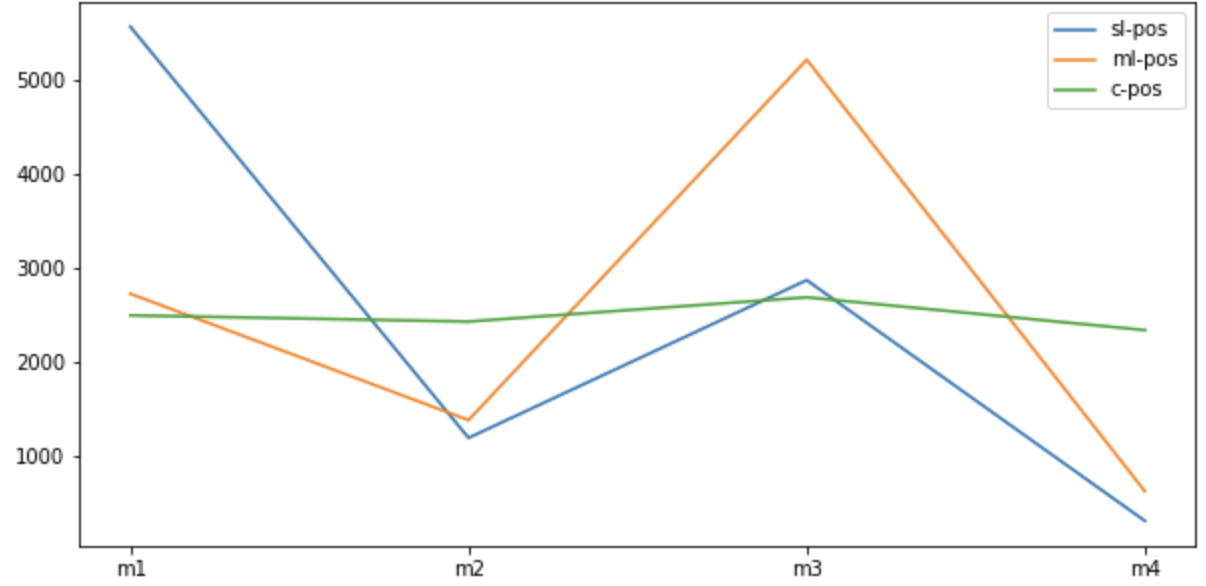
\includegraphics[width=0.7\textwidth]{stakes}
\caption{Compare the average final stake for each miner}
\label{fig:pos}
\end{figure}


And for Multi-Lottery \gls{PoS} is much better than Single-Lottery \gls{PoS}, at least the final state is related to the initial stake, if the reward for each block is smaller then Multi-Lottery \gls{PoS} can achieve robust fairness. Compare to the other two models, Compound \gls{PoS} is easier to provide robust fairness, as the final stake for each miner is almost the same even with the different initial stake power.

\section{Conclusion}
\subsection{Research question}
In conclusion our testing shows that as expected \gls{C-PoS} is both robustly and expectationally fair just like \gls{PoW} is. Addtionally it clearly showed \gls{ML-PoS} and \gls{SL-PoS} can not provide both types of fairness.

\subsection{Future work}
Given more time it would have been nice to also do the \gls{PoS} simulations in the same golang application. Also more tests with more blocks mined would have been an interesting test but this only takes time to run so it would optimally require a server to offload the work to.

\begin{thebibliography}{9}
\bibitem{paper}
Yuming Huang, Jing Tang, Qianhao Cong, Andrew Lim, and Jianliang Xu. 2021. Do the Rich Get Richer? Fairness Analysis for Blockchain Incentives. In Proceedings of the 2021 International Conference on Management of Data (SIGMOD '21). Association for Computing Machinery, New York, NY, USA, 790–803. https://doi.org/10.1145/3448016.3457285
\end{thebibliography}


\end{document}
